\documentclass[c]{beamer}
%\documentclass[c,aspectratio=1610]{beamer}
\mode<presentation>
{
  \usetheme[progressbar=frametitle]{metropolis}       % or try default, Darmstadt, Warsaw, Darmstadt ,Berkeley,...
  \usecolortheme{default} % or try albatross, beaver, crane,whale,orchid,spruce,...
  \usefonttheme{serif}    % or try default, structurebold,serif ...
  \setbeamertemplate{navigation symbols}{}
  \setbeamertemplate{caption}[numbered]
  \setbeamercovered{transparent}
} 
\addtobeamertemplate{block begin}{\pgfsetfillopacity{0.8}}{\pgfsetfillopacity{1}}
\addtobeamertemplate{block alerted begin}{\pgfsetfillopacity{0.8}}{\pgfsetfillopacity{1}}
\addtobeamertemplate{block example begin}{\pgfsetfillopacity{0.8}}{\pgfsetfillopacity{1}}

%\usepackage{beamerthemesplit}
%\usepackage[orientation=landscape,size=custom,width=14.5,height=8,scale=0.35,debug]{beamerposter}
%\usepackage[orientation=landscape,size=custom,width=18.0,height=12.0,scale=0.60,debug]{beamerposter} 

\usepackage[T1]{fontenc}
\usepackage[utf8]{inputenc}
\usepackage[brazil]{babel}
\usepackage[brazilian,hyperpageref]{backref}
\usepackage[scale=2]{ccicons}
\usepackage{pgfplots}
\usepackage{braket}
\usepackage{cancel}
%\usepgfplotslibrary{dateplot}
\usepackage{ebgaramond-maths}
%\usepackage{palatino}
%%\usepackage{kpfonts}
%\usepackage{times}
%\usepackage{xspace}
% \usepackage{natbib}
% \usepackage{cite}
\usepackage{mathtext}
\usepackage{amsfonts,amssymb}
\usepackage{amsmath,amsthm}
\usepackage{epsfig,epstopdf,url,array,latexsym}
\usepackage{graphicx}
\usepackage{mathrsfs}
\usepackage{natbib}
\usepackage{float}
\usepackage{caption}
\usepackage{subcaption}
\usepackage[mathcal]{euscript}
\usepackage{esvect}
\captionsetup[figure]{labelfont=sc}
 \usepackage{microtype} 
 \usepackage{multicol}
  \usepackage{multirow}
\usepackage{longtable}
\usepackage{lscape}
\usepackage{booktabs}
\usepackage{verbatim}
\usepackage{cprotect}
\newcommand{\themename}{\textbf{\textsc{metropolis}}\xspace}
\title{{\sc Introdução ao \LaTeX}}
%\subtitle{X Semana Acadêmica da Física\\
%	Diretório Acadêmico César Lattes}
\subtitle{Módulo I: O básico}
\date{\today}
\author{	{\large XI Semana Acadêmica da Física}\\
	Fernanda Vanucci {\sc Sica}\inst{1}\footnote{\texttt{fervanucci@gmail.com}},
	Geferson {\sc Lucatelli}\inst{1}\footnote{\texttt{gefersonlucatelli@gmail.com\\[0.5cm]}}
	}
\institute{{\Large Universidade Federal do Rio Grande} \\[0.3cm]
{\inst{1}\large Instituto de Matemática, Estatística e Física
}}
\titlegraphic{\hfill
	
\includegraphics[height=1.5cm]{images/furg.png}\\[2.5cm]{
\hspace*{8cm}
\includegraphics[height=1.5cm]{images/imef2.png}}
\hspace*{8.5cm}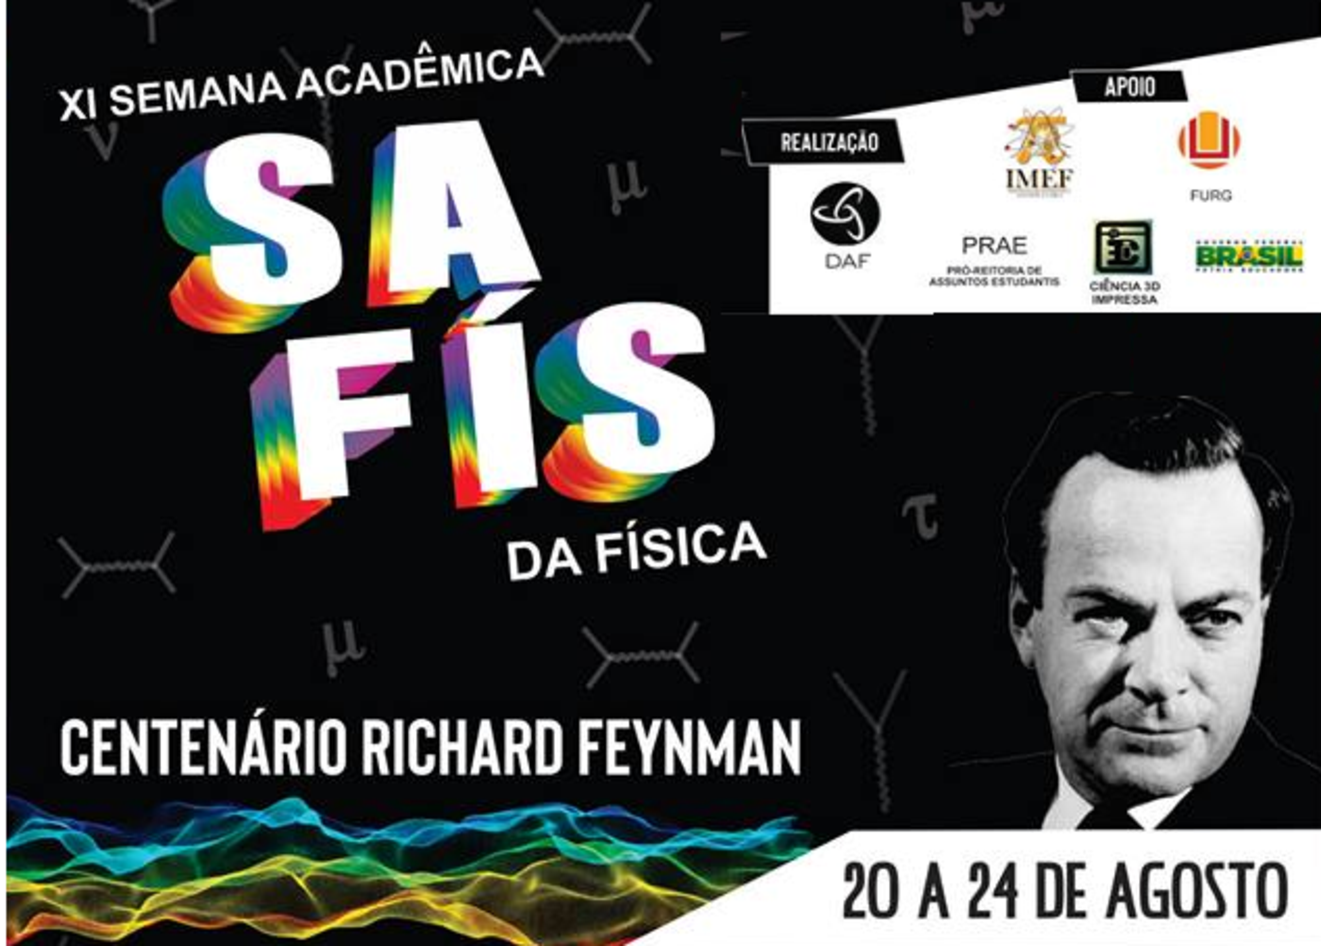
\includegraphics[height=2.0cm]{images/safis2018.pdf}
}
\newcommand{\qv}[1]{\widetilde{ #1 }}
\renewcommand{\r}{\right}
\renewcommand{\l}{\left}
\newcommand*{\EE}{\mathscr{E}}
\newcommand*{\BB}{\mathscr{B}}
\newcommand*{\Hh}{\mathscr{H}}
\newcommand*{\D}{{\rm d}}
\newcommand*{\PP}{\mathscr{P}}
\newcommand*{\WW}{\mathcal{W}}
\newcommand*{\A}{\mathscr{A}}
\newcommand{\op}[1]{\widetilde{{\bf #1 }}}
\newcommand*{\prt}{
\includegraphics[scale=0.1]{partial_symb.pdf}}%
\newcommand*{\epg}{\includegraphics[scale=0.8]{epsilon.pdf}}
\newcommand*{\ii}{\mathfrak{i}}
% \newcommand*{\prt}{\includegraphics[scale=0.40]{partial_symbol.pdf}}%
\newcommand{\source}[1]{
% \begin{flushleft}
\caption*{Fonte: {#1}} 
% \end{flushleft}
}
% \bibliographystyle{apasoft}
\bibliographystyle{apalike}
\setbeamertemplate{section in toc}{\hspace*{1em}\inserttocsectionnumber.~\inserttocsection\par}
\setbeamertemplate{subsection in toc}{\hspace*{2em}\inserttocsectionnumber.\inserttocsubsectionnumber.~\inserttocsubsection\par}
\setbeamercovered{invisible}
\usepackage{xpatch}
\usepackage{ragged2e}
\usepackage{etoolbox}
\apptocmd{\frame}{}{\justifying}{}
%\xpatchcmd{\itemize}
%{\def\makelabel}
%{\setlength{\itemsep}{5ex}\def\makelabel}
%{}
%{}
\begin{document}
\maketitle


%{\fontsize{9pt}{10.0}\selectfont

\begin{frame}{\sc Sumário}
	\begin{multicols}{2}
			\tableofcontents
	\end{multicols}
%  \setbeamertemplate{section in toc}[sections numbered]
%  \tableofcontents[section,subsection]
% \tableofcontents[hideallsubsubsections]
%   \tableofcontents[hideallsubsubsections]
\end{frame}
%}
%%%%%%%%%%%%%%%%%%%%%%%%%%%%

%\begin{frame}
%	\begin{center}
%		{\Huge Parte I}
%	\end{center}
%\end{frame}

{\fontsize{10pt}{10.0}\selectfont
%\section{Introdução as nebulosas gasosas}


\section{Motivação}
\plain{Por que utilizar \LaTeX \ como editor de texto?}

%\begin{frame}{\sc Resumo}
%		LaTeX é um editor de textos de alta qualidade tipográfica e de robusta formatação. 
%		Vem sendo muito utilizado pela academia científica mas esta se estendendo 
%		a mais áreas do conhecimento. O minicurso tem o objetivo de introduzir 
%		a linguagem LaTeX, expondo sua estrutura básica, os 
%		principais comandos utilizados, o ambiente matemático e como criar e  
%		lidar com citações e referências bibliográficas. Também será mostrado como criar e 
%		editar uma apresentação no ambiente ``beamer'' (análogo ao ``Power Point''). 
%		Além disso, o minicurso fornecerá um
%		panorama geral de maneiras para se produzir documentos científicos, tais como artigos e livros, 
%		no formato padrão das revistas de publicações.
%		Espera-se que no final do 
%		minicurso, os alunos tenham adquirido uma ideia geral do funcionamento do \LaTeX\ 
%		e que estejam aptos a criar documentos e apresentações com fórmulas 
%		matemáticas e controle de referências.
%\end{frame}
%



\begin{frame}{\sc Vantagens}
	\begin{itemize}
		\setlength\itemsep{0.2cm}
		\item \LaTeX\ permite a {\color{blue} criação} e {\color{blue} edição} de textos em variadas maneiras;
		\item possui uma alta {\color{blue} qualidade tipográfica};
		\item é eficiente na {\color{blue} organização do texto} quando ele é complexo ou grande;
		\item é a melhor ferramenta para quem precisa {\color{blue} escrever equações} (física, matemática, estatística, economia,...)!!!
		\item além disso, é muito útil para quem não trabalhe com equações, mas com {\color{blue} figuras}, 
		{\color{blue} tabelas} e qualquer tipo de {\color{blue} texto em geral};
		\item integra funções de {\color{blue} links dinâmicos} no texto, hiperlinks, etc;
		\item {\color{blue} citações} e {\color{blue} bibliografia} são gerenciados de forma automática, fácil e rápida;	
		\item reproduz o formato de grande parte de livros e artigos encontrados na literatura;
		\item possui forte {\color{blue} suporte pela comunidade};
		\item é uma {\color{blue} ferramenta livre}.
	\end{itemize}
\end{frame}
%
\begin{frame}{\sc Desvantagens (mínimas)}
	\begin{itemize}
	\setlength\itemsep{0.5cm}
	\item desvantagens estão associadas ao ``acostumar'' com a ferramenta;
	\item inicialmente, parece uma ``coisa tenebrosa'' mas com 
	algumas semanas de prática ja é suficiente para se ter uma boa habilidade no 
	uso do \LaTeX \ ;
	\item alguns dizem que digitar equações leva muito tempo, no início até certo ponto é verdade, mas 
	com o costume, tudo fica rápido. BASTA TREINAR!
	\end{itemize}
\end{frame}

\begin{frame}{\sc \LaTeX \ vs Microsoft Word (técnicas)}

	\begin{table}
		\centering
		\begin{tabular}{c|c|c} 
			\toprule
			     & \LaTeX 		& Word \\
			\midrule
			licença	       & livre		& pago\\ \hline
			\multirow{3}{*}{plataforma}	   &\multirow{1}{*}{ Linux, Windows, UNIX, } &\multirow{3}{*}{ Windows e UNIX (Mac OS)} \\ 
			&\multirow{1}{*}{ BSD, DOS, RISC OS,} &  \\ 
			&\multirow{1}{*}{ AmigaOS e Plan9} &  \\ \hline
			ferramenta online & idêntica ao desktop & limitada\footnote{Veja \url{http://sharepointmaven.com/office-online-sharepoint-onedrive/}.}  \\ \hline
			\bottomrule
		\end{tabular}
		% \source{Elaborado pelo autor.}
		\caption{}
		\label{a_b_values_tab}
	\end{table}

\end{frame}

\begin{frame}{\sc \LaTeX \ vs Microsoft Word (estética)}
\begin{figure}[b!]
	\centering
	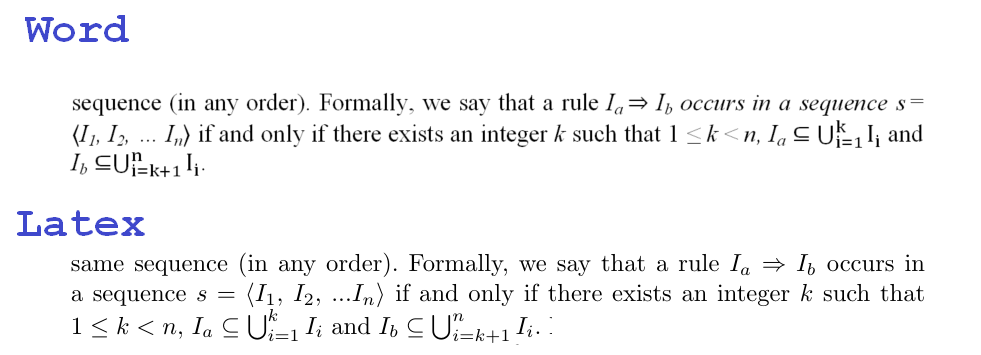
\includegraphics[width=0.99\linewidth]{images/word_vs_latex.png}
	\caption{Fonte: \url{http://data-mining.philippe-fournier-viger.com}.}
	\label{latex_vs_word}
\end{figure}
\end{frame}

\begin{frame}{\sc \LaTeX \ vs Microsoft Word (eficiência)}
	\begin{figure}[b!]
		\centering
		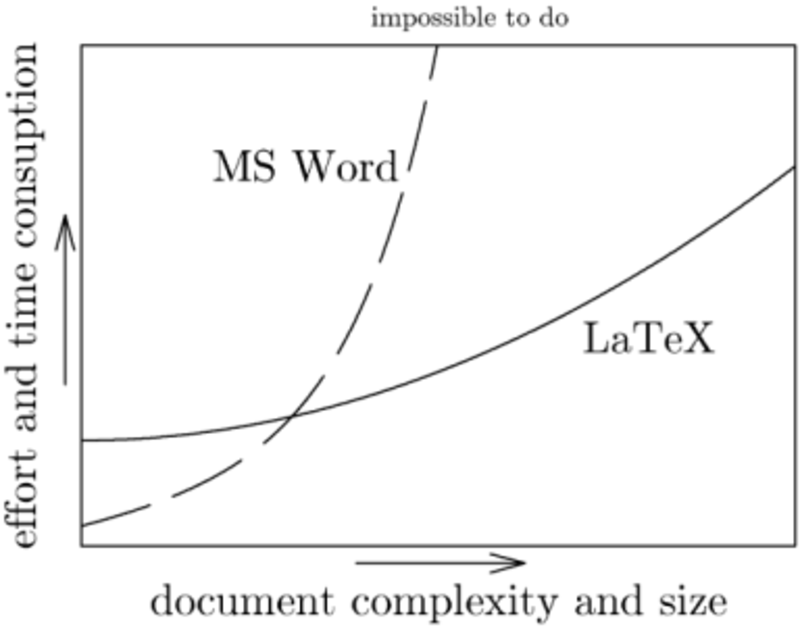
\includegraphics[width=0.59\linewidth]{images/wordvslatex.pdf}
		\caption{Fonte: \url{https://www.johndcook.com/wordvslatex.gif}.}
		\label{latex_vs_word2}
	\end{figure}
\end{frame}

\plain{E aí, foi convencido?}

\section{Instalação}

\begin{frame}{\sc Usuários Linux (recomendado)}
\begin{itemize}
	\setlength\itemsep{0.2cm}
	\item instalando a biblioteca:
	\begin{itemize}
	\item[$\to$] abra o terminal (Ctrl+Alt+T) e digite:\\
	 \texttt{sudo apt install texlive-full}
\end{itemize}
	\item instalando o compilador e visualizador de pdf:
	\begin{itemize}
		\item[$\to$] há três compiladores muito usados:  TexStudio (recomendado), Kile e  TexMaker:\\
		\texttt{sudo apt install texstudio} ou \texttt{kile} ou \texttt{texmaker}
		\item[$\to$] o TexStudio e o TexMaker possuem um visualizador embutido. Outras opções são Okular, FoxitReader ou AdobeReader;
		\item[$\to$] para instalar o okular:\\
		\texttt{sudo apt install okular}
	\end{itemize}
	\item pronto!!!
\end{itemize}
\end{frame}

\begin{frame}[fragile]{\sc Usuários Windows}
	Para a instalação do \LaTeX\ no Windows, basta fazer o download e instalação de:
	\begin{itemize}
		\setlength\itemsep{0.3cm}
		\item Texmaker:  \url{http://cluster.ft.unicamp.br/wiki/doku.php?id=ambiente:latex_windows};
		\item baixe a versão correta para seu computador;
		\item baixar o \TeX\ Live: \url{https://www.tug.org/texlive/acquire-netinstall.html} em \emph{install-tl-windows.exe} \quad $\sim$ \quad 4.4 Gb
	\end{itemize}
\end{frame}

\section{Conhecendo o compilador}
\subsection{Texstudio}
\plain{Vejamos o compilador Texstudio.}


\section{Estrutura de um documento}


\plain{O primeiro passo é conhecer a estrutura de um documento}

\begin{frame}[fragile]{\sc Estrutura de um documento: preâmbulo e corpo}
	Um documento (\verb|.tex|) em \LaTeX\ é composto basicamente de duas partes:
	\begin{itemize}	
		\setlength\itemsep{0.2cm}
		\item o {\color{blue} preâmbulo}  contém 
		todas as configurações do texto a ser criado, são feitas as declarações sobre a {\color{blue} classe} do documento, 
		{\color{blue} configurações globais} e o carregamento dos {\color{blue} pacotes}. 
        É possível criar somente um documento para este fim - o 
		{\color{blue} documento mestre} (veremos adiante);
		\item {\color{blue} corpo}: contém o texto propriamente dito;
	\end{itemize}
\end{frame}


\subsection{Preâmbulo}

\begin{frame}[fragile]{\sc Preâmbulo: classe (\texttt{documentclass})}
	\begin{itemize}
		\setlength\itemsep{0.2cm}
		\item a {\color{blue} classe} de um documento é o modelo de texto a ser criado:
		\begin{verbatim}
		\documentclass[options]{class}
		\end{verbatim}
  \item As {\color{blue} opções} se referem às seguintes configurações:
  \begin{itemize}
  	\item tamanho da fonte do texto (\verb|10pt|, \verb|12pt|, \verb|14pt|);
  	\item formato do papel (\verb|a4paper|);
  	\item número de colunas (\verb|onecolumn|, \verb|twocolumn|);
  	\item orientação da folha (\verb|landscape|, \verb|portrait|);
  	\item impressão só frente ou frente e verso (\verb|oneside|, \verb|twoside|);
  \end{itemize}
    \end{itemize}
\end{frame}


\begin{frame}[fragile]{\sc Preâmbulo: classe (\texttt{documentclass})}
Aguns tipos de classe são:
	\begin{itemize}
	\setlength\itemsep{0.2cm}
	\item \verb|article| : Artigos científicos, documentos curtos, relatórios, etc.
	\item \verb|beamer| : Apresentações latex.
	\item \verb|book| : Livros.
	\item \verb|letter| : Cartas.
	\item \verb|report| : Livros pequenos, teses, relatórios longos, etc.
\end{itemize}
Essas apresentações usam \verb|\documentclass{beamer}|. O estudo dessa classe será visto no Módulo III.
\end{frame}


\begin{frame}[fragile]{\sc Preâmbulo: pacotes (\texttt{usepackage})}
	\begin{itemize}
		\setlength\itemsep{0.2cm}
		\item os {\color{blue} pacotes} são as ferramentas da base \TeX\ a serem {\color{blue} importados} de acordo com 
		a {\color{blue} necessidade} do texto;
		\item  a {\color{blue} declaração} dos pacotes é feita através do {\color{blue} comando}:
		\begin{verbatim}
		\usepackage[options]{package}
		\end{verbatim}
		\item {\color{blue} exemplos} de pacotes importantes:
    \begin{itemize}
    	\item \verb|babel|: Pacote para {\color{blue} hifenização} automática e modificação das {\color{blue} regras tipográficas} do texto. 
    	Para usar português do Brasil, usamos \texttt{brazil} como opção;
    	\item \verb|inputenc|: \emph{{\color{blue} encoding}} utilizado na fonte do documento. 
    	Caracteres com {\color{blue} acentos} podem ser digitados diretamente no código fonte. 
    	As opções mais usadas são o \verb|utf8| e o \verb|latin1|;
    	\item \verb|amssymb|, \verb|amsmath|: Habilitam alguns {\color{blue} caracteres} e {\color{blue} comandos matemáticos} especiais.
    	\item \verb|geometry|: Pacote para configurar as dimensões das {\color{blue} margens} e {\color{blue} largura}
    	da folha;
		\item \verb|graphicx|: utilizado para inserir {\color{blue} figuras};
		\end{itemize}
	\end{itemize}
\end{frame}


\subsection{Corpo}

\begin{frame}[fragile]{\sc Corpo: \texttt{document}}
	\begin{itemize}
		\setlength\itemsep{0.3cm}
   \item o {\color{blue} corpo do documento} consiste em tudo aquilo que está inserido entre os
   seguintes comandos:\\
   \begin{center}
   	\verb| \begin{document} |\\
   	.\\
   	.\\
   	.\\
   	\verb| \end{document} |
   	\end{center}
   	\item todos os capítulos, seções e subseções devem estar inseridos entre estes
   	comandos; 
   	\item o que for escrito após o fim do documento será ignorado pelo compilador.
		\end{itemize}
\end{frame}



\begin{frame}[fragile]{\sc Corpo: organização}
	\begin{itemize}
		\setlength\itemsep{0.3cm}
		\item se você for criar um texto grande, é ideal que se mantenha uma {\color{blue} organização 
		dos arquivos}. 
		\begin{center}
			\underline{Quais arquivos?}
		\end{center}
		\item por exemplo, se for criado um documento com $x$ capítulos, a dica é criar para cada capítulo uma 
		pasta e nessa coloque todos os arquivos referentes ao capítulo;
		\item o mesmo se aplica para arquivos de figuras;
	\end{itemize}
\end{frame}


\begin{frame}[fragile]{\sc Corpo: organização}
	\begin{itemize}
		\setlength\itemsep{0.3cm}
		\item crie um {\color{blue} documento mestre}. Esse é constituído do preâmbulo com os 
		pacotes $+$ o corpo, entretanto não escreva nenhum texto no corpo;
		\item ao invés, dentro do \verb|document| (que é o corpo) {\color{blue} importe os arquivos} que contém o {\color{blue} texto} utilizando 
		os comandos \verb|\input{pasta_1/texto_1}| ou \verb|\include{pasta_1/texto_1}|;
		\item por exemplo
		\begin{verbatim}		
		\begin{document}
		\include{prefacio/prefacio}
		\input{capitulo_1/capitulo_1}
		\input{capitulo_2/capitulo_2}		
		\end{document}
		\end{verbatim}
	\end{itemize}
\end{frame}

\begin{frame}[fragile]{\sc O pacote subfile}
  \begin{itemize}
   \setlength\itemsep{0.3cm}
   \item O pacote {\color{blue} \verb|subfile|}, assim como  {\color{blue}\verb|\input|} e  {\color{blue}\verb|\include|}, permite a modularização do documento.
   \item Para ser utilizado basta adicionar ao preâmbulo e chamar o arquivo com:\\
   \verb|\subfile{}|\\
         E o subarquivo deve conter:\\
   \verb|\documentclass[diretório do main/main.tex]{subfiles}|\\
   \item Sua principal vantagem é que os subarquivos são arquivos \verb|.tex| o que              permite sua compilação separada do arquivo principal, sem ser necessário                compilar todos os documentos ao mesmo tempo. 
   \item Ideal para documentos grandes, como teses e livros, com multiplos capítulos.
   \item Sua principal desvantagem é que para que o pacote {\color{blue}\verb|graphicx|}          funcione normalmente é necessário informar o diretório relativo das imagens em          relação ao documento principal e ao subarquivo:\\
   \verb|\grapichspath{{images/}{../images}}|
  \end{itemize}
\end{frame}

\section{Formatação de texto}

\plain{Começando a digitar textos...}

\subsection{Comandos de texto}
\begin{frame}[fragile]{\sc Comandos de texto}
	\begin{itemize}
		\setlength\itemsep{0.5cm}
		\item o \LaTeX é estruturado a base de {\color{blue} comados} e {\color{blue} sintaxes}, 
		porém todos relativamente simples;
		\item {\color{blue} palavras} são separadas por espaços em branco;
		\item todo {\color{blue} comando} inicia com um \emph{{\color{blue} backslash}} \verb|\|;
%		\item exemplos de comandos básicos:
%		\begin{itemize}
%			\item para fonte itálica $\quad \to \quad$ \verb|\emph{texto}| $\quad$ produz $\quad$ \emph{texto};
%			\item para negrito $\quad \to \quad$ \verb|\textbf{texto}| $\quad$ produz \textbf{texto};
%		\end{itemize}
		\item {\color{blue} comentários} no editor são criados com \verb|%|. Qualquer caractere preenchido com
		\verb|%| não aparecerá no arquivo \verb|.pdf|;
		\item {\color{blue} caracteres especiais do \LaTeX\ }:\verb|%|, \verb|#|, \verb|&| e \verb|$|. 
		Se quiser usá-los como texto, deve usar \verb|\| à esquerda, por exemplo \verb|\%|, etc;
		\item caracteres matemáticos são incluídos no texto entre dois símbolos \verb|$|;
%		\item use frequentemente \verb|{| e \verb|}| para 
	\end{itemize}
\end{frame}



\begin{frame}[fragile]{\sc O uso de \texttt{\$}}
	\begin{itemize}
		\setlength\itemsep{0.3cm}
		\item o {\color{blue} símbolo \verb|$|} é utilizado para marcar {\color{blue} caracteres matemáticos} no texto;
	\begin{table}[h]
		\begin{tabular}{|l|} 
			%		\toprule
			\hline
			Seja $a$ e $b$ definidos pela relação: $a+b=1$. \\ \hline
			\verb|Seja $a$ e $b$ definidos pela relação: $a+b=1$.| \\ \hline
			%		\midrule
		\end{tabular}
	\end{table}
	\item veremos mais sobre seu uso adiante;
\end{itemize}
\end{frame}


\begin{frame}[fragile]{\sc Exercício de texto simples}
	Reproduza o texto a seguir:\\[0.5cm]
``O nosso orçamento para 2017 aprovado pelo Congresso e mais 
o Fundo Nacional de Desenvolvimento Científico e Tecnológico 
previstos para este ano estavam suficientes para que 
tocássemos 2017 com tranquilidade", diz o presidente do CNPq, 
Mario Neto Borges. No total, o Orçamento previa R\$ 1,3 bilhão 
e o fundo, R\$ 400 milhões à autarquia - 44\% desses valores 
foram contingenciados. Do fundo, o CNPq recebeu menos do que 
56\%: até o momento o valor pago foi R\$ 62 milhões.''

Fonte: Agência Brasil
\href{http://agenciabrasil.ebc.com.br/educacao/noticia/2017-08/apos-corte-de-verbas-cnpq-tem-recursos-para-pagar-bolsas-apenas-ate-este}{(link)}
\end{frame}


\begin{frame}[fragile]{\sc Exercício de texto simples (solução)}
			\begin{verbatim}
O nosso orçamento para 2017 aprovado pelo Congresso e mais 
o Fundo Nacional de Desenvolvimento Científico e Tecnológico 
previstos para este ano estavam suficientes para que 
tocássemos 2017 com tranquilidade", diz o presidente do CNPq, 
Mario Neto Borges. No total, o Orçamento previa R\$ 1,3 bilhão 
e o fundo, R\$ 400 milhões à autarquia - 44\% desses valores 
foram contingenciados. Do fundo, o CNPq recebeu menos do que 
56\%: até o momento o valor pago foi R\$ 62 milhões.
			\end{verbatim}
\end{frame}

\plain{Formatação e ajuste de texto.}
\subsection{Formatação e ajuste de texto}

\begin{frame}[fragile]{\sc Formatação: justificação e hifenização}
	\begin{itemize}
		\setlength\itemsep{0.3cm}
		\item no \LaTeX, o texto é {\color{blue} justificado automaticamente}; 
		\item a opção \verb|brazil| do pacote \verb|babel| trata de {\color{blue} hifenizar automaticamente} as palavras 
		para nova linha no idioma PT-BR;
	\end{itemize}
\end{frame}

\begin{frame}[fragile]{\sc Formatação: negrito, itálico, sublinhado e outros}
	\begin{itemize}
		\setlength\itemsep{0.3cm}
\item {\color{blue} Negrito}: \verb|\textbf{Texto}| ou \verb|{\bf Texto }| produz \textbf{Texto}
\item {\color{blue} Itálico}: \verb|\textit{Texto}| ou \verb|\emph{Texto}| produz \textit{Texto}
\item {\color{blue} Sublinhado}: \verb|\underline{Texto}| produz \underline{Texto}
\item {\color{blue} Letra de código}: \verb|\texttt{Texto}| produz \texttt{Texto}
\item {\color{blue} Fonte \verb|sc|} para títulos: \verb|{\sc Título}| ou \verb|\textsc{}| produz {\sc Título};
\item {\color{blue} alterando a cor}: \verb|{\color{blue} Texto}| produz {\color{blue} Texto};
%\item Caixa alta: \verb|\textsc{Texto}| produz \texts 
	\end{itemize}
OBS: Note o uso frequente de \verb|{}| para delimitar a região de atuação de um dado comando! Dessa maneira 
\{ \} não é inserido no texto, para isso utilize \verb|\{ \}|.
\end{frame}


\begin{frame}[fragile]{\sc Formatação: tamanho e tipo da fonte}
	\begin{itemize}
		\setlength\itemsep{0.3cm}
		\item o {\color{blue} tamanho do texto} é modificado de acordo com o apresentado abaixo:
	\begin{table}[h]
		\begin{tabular}{|l|l|} 
			%		\toprule
			\hline
			\verb|{\tiny Texto}| & {\tiny Texto} \\ \hline
			\verb|{\scriptsize Texto}| & {\scriptsize Texto} \\ \hline
			\verb|{\footnotesize Texto}| & {\footnotesize Texto} \\ \hline
			\verb|{\small Texto}| & {\small Texto} \\ \hline
			\verb|{\normalsize Texto}| & {\normalsize Texto} \\ \hline
			\verb|{\large Texto}| & {\large Texto} \\ \hline
			\verb|{\Large Texto}| & {\Large Texto} \\ \hline
			\verb|{\LARGE Texto}| & {\LARGE Texto} \\ \hline
			\verb|{\huge Texto}| & {\huge Texto} \\ \hline
			\verb|{\Huge Texto}| & {\Huge Texto} \\ \hline
		\end{tabular}
	\end{table}
	\item uma {\color{blue} generalização} para o tamanho e espaçamento (das linhas) é obtida com o comando 
	\verb|{\fontsize{12pt}{10.0}\selectfont Texto}| (12 é o tamanho e 10 o espaçamento).
		\end{itemize}
\end{frame}

\begin{frame}[fragile]{\sc Formatação: espaçamento}
O \LaTeX \ manipula os {\color{blue} espaçamentos automaticamente}, 
porém nem sempre o documento compilado fica do formato desejado. 
Portanto, existem alguns comandos para {\color{blue} manipular os espaçamentos}.
	\begin{itemize}
		\setlength\itemsep{0.3cm}
\item \verb|\hspace{tamanho}| produz espaçamento horizontal
\item \verb|\vspace{tamanho}| produz espaçamento vertical
\item \verb|\\[tamanho]| produz espaçamento vertical antes de começar uma nova linha
\end{itemize}
Estes três comandos acima necessitam da {\color{blue} opção} \texttt{tamanho} que é definido pelo usuário. 
Esta opção deve ser um {\color{blue} número} seguido de sua {\color{blue} unidade}. Por exemplo,
\begin{itemize}
		\setlength\itemsep{0.3cm}
	\item \verb| \hspace{5cm}|
	\item \verb| \\[8mm]|
	\end{itemize}
\end{frame}


\begin{frame}[fragile]{\sc Formatação: espaçamento}
	Existem {\color{blue} outros comandos} que não necessitam de um tamanho especificado pelo usuário:
	\begin{itemize}
		\setlength\itemsep{0.3cm}
\item \verb|\hfill| adiciona espaços horizontais para preencher a largura da pagina
\item \verb|\vfill| adiciona espaços verticais para preencher a altura da pagina
\item \verb|\newline| inicia uma nova linha
\item \verb|\newpage| inicia uma nova página
\item \verb|\noindent| remove o espaçamento antes do parágrafo.
	\end{itemize}
\end{frame}

\begin{frame}[fragile]{\sc Formatação: espaçamento}
No \LaTeX \ também é possível modificar o {\color{blue} espaçamento entre linhas}. 
Há mais de uma forma de modificar este espaçamento. Para isto, teremos que adicionar ao preambulo o pacote:
\begin{verbatim}
\usepackage{setspace}
\end{verbatim}
O espaçamento pode ser modificado utilizando os comandos:
	\begin{itemize}
		\setlength\itemsep{0.3cm}
\item \verb|\singlespacing| espaçamento simples entre linhas 
\item \verb|\onehalfspacing| espaçamento $1.5$
\item \verb|\doublespacing| espaçamento duplo
	\end{itemize}
Também é possível utilizar 	 o comando 
\begin{verbatim}
\renewcommand{\baselinestretch}{1.0}
\end{verbatim}
(troque $1.0$ pelo espaçamento 
desejado).
\end{frame}


\begin{frame}[fragile]{\sc Formatação: Fontes}
	\begin{itemize}
		\setlength\itemsep{0.3cm}
		\item é possível {\color{blue} trocar} a fonte de todo documento. A troca 
		é realizada com a adição do respectivo pacote de cada fonte;
		\item algumas fontes disponíveis que suportam o ambiente matemático são:
		\begin{enumerate}[$\to$]
			\item padrão: \verb|cmr| (não é preciso pacote);
			\item Arev Sans: pacote \verb|arev|;
			\item garamond: pacote \verb|ebgaramond-maths|;
			\item palatino: pacote \verb|palatino|;
			\item times: pacote \verb|times|;
			\item CM Bright: pacote \verb|cmbright|;
			\item Concrete Font: \verb|ccfonts|;
			\item Kurier: pacote \verb|kurier| com a opção \verb|math|;
		\end{enumerate}
		\item entre outros\footnote{Veja a lista completa em \url{http://www.tug.org/pracjourn/2006-1/hartke/hartke.pdf}.}.
	\end{itemize}
\end{frame}


\plain{Secionando o documento}
\subsection{Secionando o documento}

\begin{frame}[fragile]{\sc Hierarquia do documento: parte, capítulo, seções,...}
Todo texto é organizado/dividido por {\color{blue} capítulos}, {\color{blue} seções}, etc, e essa {\color{blue} divisão} é 
{\color{blue} enumerada}. No \LaTeX, 
todas as enumerações são {\color{blue} automáticas} e essa é a grande vantagem. 
No \LaTeX \ títulos e subtítulos são chamados de \texttt{section} e \texttt{subsection}.
A {\color{blue} divisão hierárquica} completa é:
	\begin{itemize}
		\setlength\itemsep{0.3cm}
		\item o 1º grau hierárquico de um documento é a parte: \verb|\part{Título da Parte}|;
		\item o 2º grau hierárquico de um documento é o capítulo: \verb|\chapter{Título da Parte}| (é claro, exeto para classes que por definição não o possuem, por exemplo \verb|article|);
		\item o 3º grau é a seção: \verb|\section{Seção 1}|;
		\item o 4º grau é a subseção: \verb|\subsection{Subseção 1}|
		\item o 5º grau é a subsubseção: \verb|\subsubsection{Subsubseção 1}|
		\item o 6º grau é o parágrafo: \verb|\paragraph{Parágrafo 1}|
	\end{itemize}
Para {\color{blue} remover a enumeração}, basta utilizar * após o comando de título, 
por exemplo: \verb|\section*{Título}|;
\end{frame}

\begin{frame}[fragile]{\sc Hierarquia do documento: parte, capítulo, seções,...}
\center{Exemplo de títulos:}
\vspace{0.2cm}
\begin{columns}
	\begin{column}{0.4\textwidth}
		%\centering
		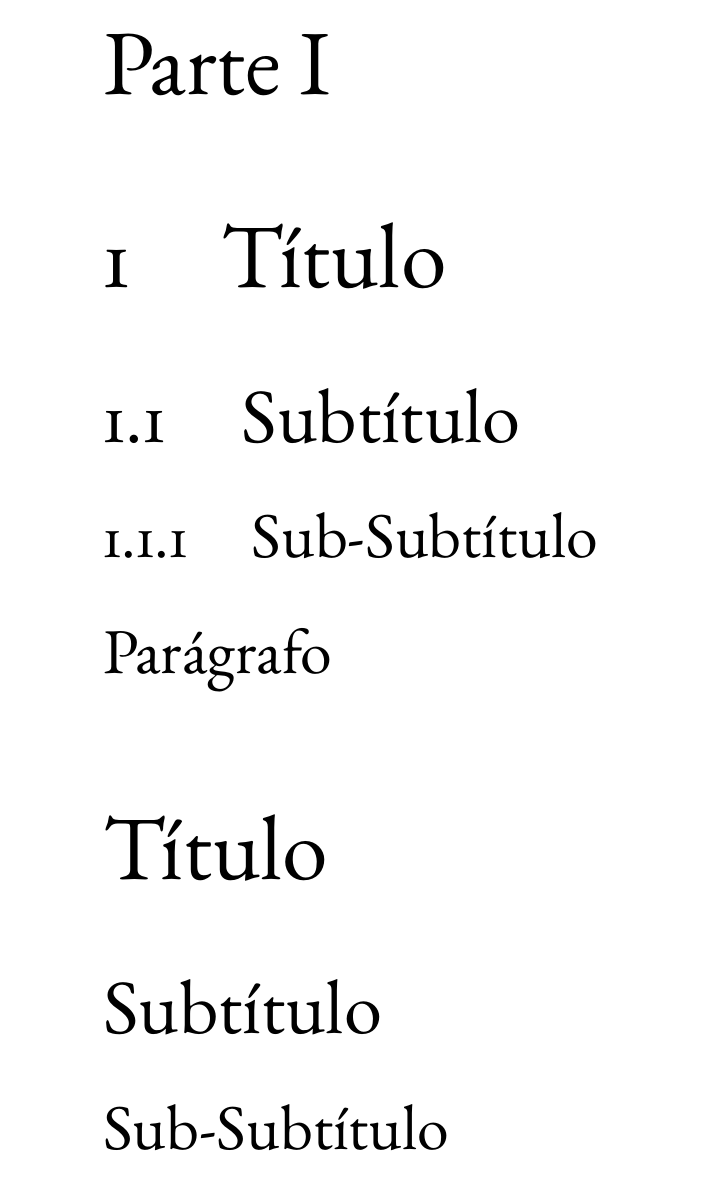
\includegraphics[scale=0.2]{images/exemplo_titulos.png}
		\end{column}
		%
		\begin{column}{0.6\textwidth}
		\begin{verbatim}
\part{}
\section{Título}
\subsection{Subtítulo}
\subsubsection{Sub-Subtítulo}
\paragraph{Parágrafo}
\section*{Título}
\subsection*{Subtítulo}
\subsubsection*{Sub-Subtítulo}
		\end{verbatim}
		\end{column}
			
			\end{columns}
			
\end{frame}



\section{Exercício com a classe \texttt{article}}


\plain{O básico do \LaTeX\ já temos em mãos.\\
	Vamos começar a editar um texto simples!!}

\plain{Exemplo simples utilizando a classe \texttt{article}}


%\begin{frame}[fragile]{\sc Criando o preâmbulo da classe article}
%	\begin{itemize}
%		\setlength\itemsep{0.5cm}
%		\item o preâmbulo contém todas as configurações necessárias para editar 
%		o seu texto desejado: espaçamento, fonte, tamanho, etc;
%		\item para isso, pacotes da base \LaTeX\ são importados: \verb|\usepackage[opções]{package}|:
%		\item por exemplo, para inserir figuras, é preciso importar o pacote 
%		\verb|\usepackage{graphicx}|;
%	\end{itemize}
%\end{frame}
%
%\begin{frame}[fragile]{\sc 1º Passo: Classe do documento}
%	\begin{itemize}
%		\setlength\itemsep{0.5cm}
%		\item classe de documento a ser criado:
%		\begin{verbatim}
%		\documentclass[opções]{tipo de documento}
%		\end{verbatim}
%		\item \verb|opções: tamanho da fonte, tamanho do papel, ....|;
%		\item \verb|tipo: article, book, beamer, report,...|
%		\item cada classe permite editar um layout em específico;
%		\item essas apresentações usam \verb|\documentclass{beamer}|;
%	\end{itemize}
%\end{frame}


\begin{frame}[fragile]{\sc Exemplo \texttt{article}}
\begin{verbatim}
\documentclass[12pt,a4paper]{article}
\usepackage[T1]{fontenc}
\usepackage[brazil]{babel}
\usepackage[utf8]{inputenc}
\usepackage{amssymb,amsmath}
\end{verbatim}
\end{frame}

\begin{frame}[fragile]{\sc Exemplo \texttt{article}}
\begin{itemize}
	\setlength\itemsep{0.5cm}
	\item após a importação dos pacotes, começamos editando o documento;
	\item {\color{blue} título} e {\color{blue} autor} são criados com \verb|\title{título}| e \verb|\author{autor}|, respectivamente;
	\item a {\color{blue} data} é inserida automaticamente, caso contrário, use \verb|\date{data}| ou 
    \verb|\date{\today}|;
	\item insira esses elementos após o \verb|\begin{document}|;
	\item para criar esses elementos no \verb|.pdf|, insira o comando \verb|\maketitle| logo em seguida;
\end{itemize}
\end{frame}


\begin{frame}[fragile]{\sc Exercício}
	Como um exercício, crie um documento \verb|.tex| para a classe \verb|article|. 
	\begin{itemize}
		\setlength\itemsep{0.3cm}
		\item adicione os pacotes a serem utilizados (copiem e colem o que já digitaram até agora);
		\item insiram as informações do título, autor e data;
		\item façam um pequeno texto, dividido por seções e subseções com o que foi aprendido até agora,
		formatação (negrito, itálico, tamanho, espaçamento, ...)
	\end{itemize}
\end{frame}


\begin{frame}[fragile]{\sc Exercício}
\begin{verbatim}
\documentclass[12pt,a4paper]{article}
\usepackage[T1]{fontenc}
\usepackage[brazil]{babel}
\usepackage[utf8]{inputenc}
\usepackage{amssymb,amsmath}
\usepackage{graphicx}

\begin{document}

\title{Minicurso \LaTex}
\autor{X Semana Acadêmica da Física}
%\date{}

\maketitle

texto a ser inserido aqui...
\end{document}
\end{verbatim}
\end{frame}

\plain{Fim do Módulo I!!!\\
Dúvidas? }
%\section{Referências}



\begin{frame}[allowframebreaks]{References}
\bibliography{references}
\nocite{*}
\end{frame}

\begin{frame}[fragile]{\sc Links úteis}
	Curso online de \LaTeX\ \href{https://www.overleaf.com/latex/learn/free-online-introduction-to-latex-part-1#.WZxOyXV97-c}{aqui}.\\[2cm]
	
	Livro extenso sobre \LaTeX\ \href{https://upload.wikimedia.org/wikipedia/commons/2/2d/LaTeX.pdf}{aqui}.
\end{frame}

\plain{Gracie!}

} 

\end{document}


